\chapter{\MakeUppercase{Моделирование ходьбы}}
\section{Траектории движения ног}

Самым простым способом реализации ходьбы является такой, при котором робот по очереди переставляет ноги в нужном порядке, всегда имея три точки опоры. Было решено реализовать модернизированную версию такого способа перемещения. Модернизация заключается в том, что ноги двигаются непрерывно, из-за чего робот будет периодически опираться не на три, а на две точки.

Движение ноги во время ходьбы было описано при помощи двух замкнутых траекторий движения точки $ A $ в двух проекциях: на плоскость $ XZ $ и $ XY $. На полученных траекториях берется множество точек, в которые по очереди переносится точка $A$ робота управляющей программой.

В качестве первого приближения для траектории в проекции на плоскость $ XZ $ был выбран эллипс, для траектории в проекции на плоскость $ XY $ выбрана <<линия>> (эллипс с нулевой малой полуосью), по которой точка $ A $ будет периодично двигаться то в одном, то в другом направлении.

[Иллюстрация]

Точки на этих траекториях достаточно легко вычислять для каждого момента времени, если кривые описаны функцией. Следует отметить, что на практике абсолютный энкодер установленный в подобранных приводах имеет <<область нечувствительности>> (рисунок \ref{fig:nonff}). Это приводит к тому, что при слишком малом расстоянии между точками, выбранными на траектории, текущая и новая конфигурации ног слабо отличаются. Это в свою очередь приводит к тому, что двигатели просто <<игнорируют>> управляющий сигнал, сообщающий о необходимости поворота на новый, слабо отличающийся угол. Упрощенная схема работы сервопривода показана на рисунке \ref{fig:upr_servo}.

\begin{figure}[h]
    \centering
    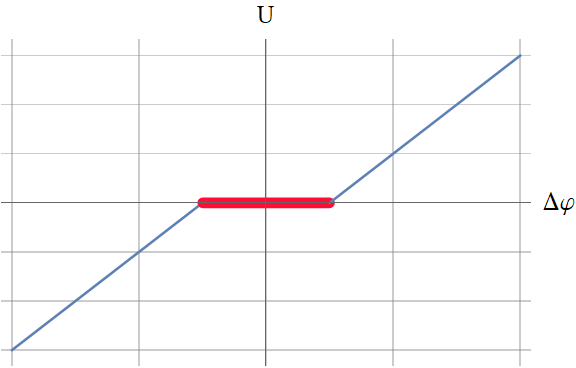
\includegraphics[scale=0.6]{chapter_walking_model/figure2.png}
    \caption{Область нечувствительности отмечена красным цветом}
    \label{fig:nonff}
\end{figure}

\begin{figure}[h]
    \centering
    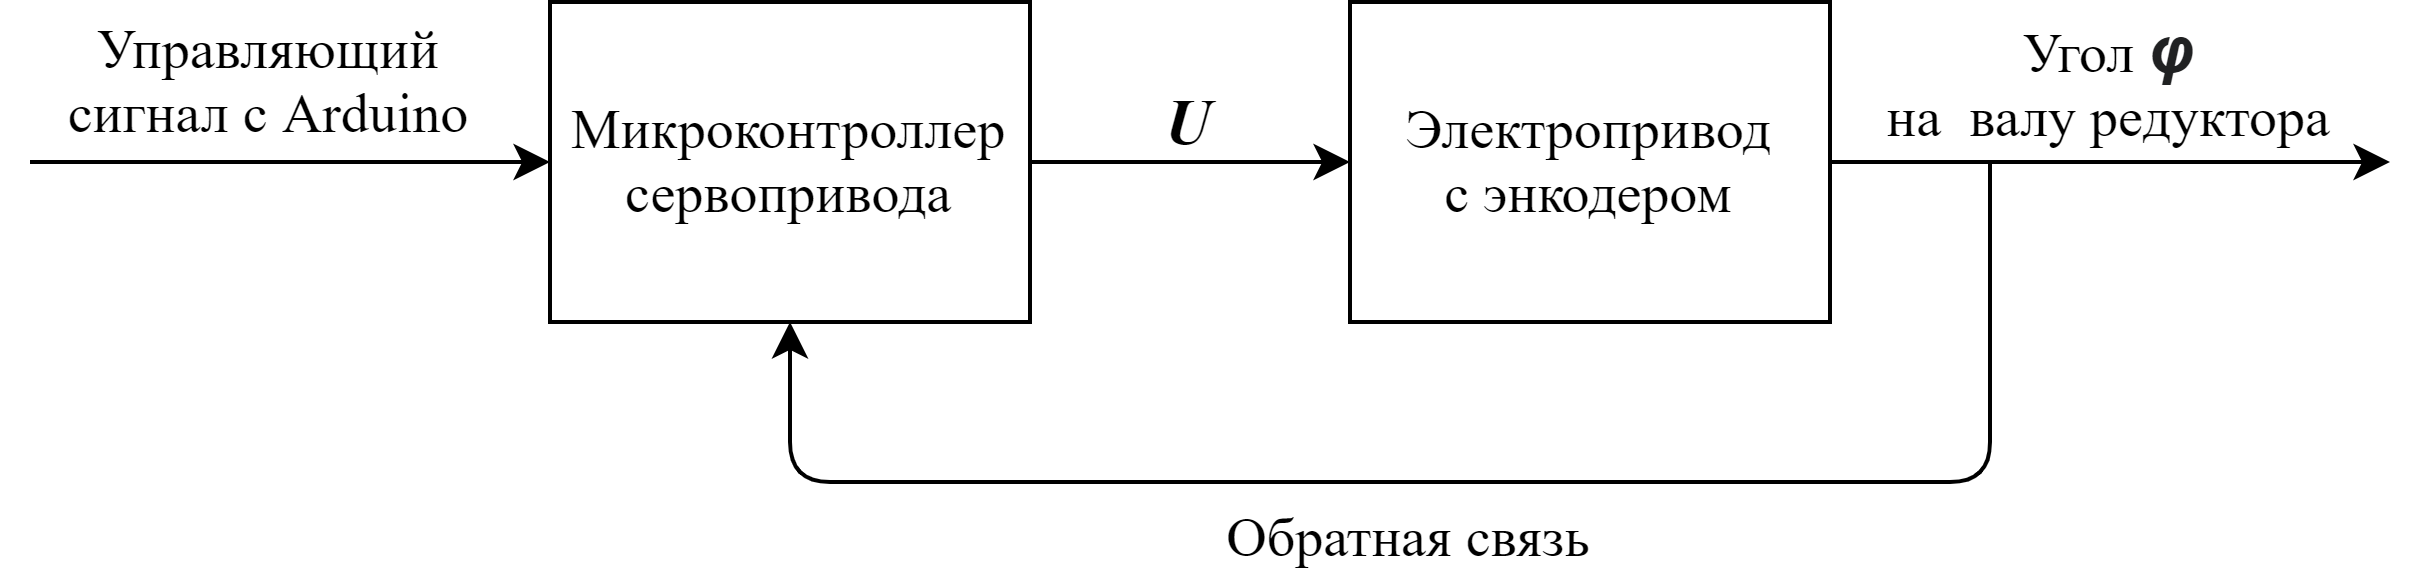
\includegraphics[width=\textwidth]{chapter_walking_model/figure1.png}
    \caption{Упрощенная схема внутренней системы управления сервопривода}
    \label{fig:upr_servo}
\end{figure}

Чем меньше точек мы берем на траектории, тем менее точно конечность описывает нужную нам траекторию, что наглядно показано на иллюстрации [].

[иллюстрация]

Экспериментальным путем был найден результат, максимально удовлетворяющий на практике.


\section{Проблема выбора оптимальной траектории}

Эллипс не является оптимальной траекторией, обычно требуются траектории более сложные, не всегда выпуклые \cite{Singla2018}. 